\documentclass[11pt]{article}
\usepackage{fullpage}
\usepackage{cite}
\usepackage{datetime}
\usepackage{geometry}
\usepackage{graphicx}
\geometry{verbose,lmargin=3cm,rmargin=3cm}

\title{Automated negotiation in the game of diplomacy - Report 3: Overview and Software Validation}
\author{Matthias Hueser, Andras Slemmer, Luca Deltodesco, Luke Tomlin, Cliff Sun}
\date{\today}

\begin{document}
\maketitle

\section{Project synopsis}
The Game of Diplomacy is a round-based multiplayer strategy-game set in post WWI
Europe. Each player controls a power which initially operates from a number of 
home-bases. The ultimate objective of each player is to control the majority of
supply-centers on the map. A game is structured into a number of rounds, in which
each player formulates a move order to conquer additional supply centres or
defend existing ones. Besides the necessity to create effective long-term
strategies negotiation is integral to the game-experience. There is a thriving
internet-based community around the Game of Diplomacy and many AI players, so
called bots, have been created in the past. Most of the existing AI players are
quite effective decision-makers in general but few of them support negotiation
or reasoning about the relationship of the powers in the game. Our projects aim
to create a framework for Diplomacy, including a GUI client, a game server and a
collection of bots. Crucially one the bots or the highest evolution of our series
of bots should be able to analyze and act upon messages of human / AI players.
Then experiments are run to determine whether there is a reward associated with
negotation capabilities. This will require careful study and implementation of
automated negotiation techniques from other domains. Hence the project gives us
ample opportunity to be creative and test different approaches using the
DAIDE-conforming game framework produced for the project. DAIDE is a standard
client-server protocol which serves as a 'common language' for different Diplomacy
bot implementations, enabling them to play a game together on a conforming
server.

\subsection{Requirements engineering / management}
High-level requirements were discussed in the initial phase of the project 
(weeks 1/2) with our project supervisor -- Iain Philipps -- who was our customer
in Software Engineering terms. The terms of the collaboration were such that 
only certain high-level goals were defined and project metrics were defined: 

\begin{itemize}

\item The over-arching goal and hence the most critical requirement is to 
      design and implement a negotiation bot for Diplomacy whose performance
      is then compared to existing bots in an experimental setting. 
\item A collection of other bots which are not capable of commuication should
      be created for purposes of comparison. These should use proven techniques
      from the fields of Game Theory and Multi-Agent systems, including learning,
      tactics and long-term strategies. All bots should support the DAIDE 
      protocol to compete against existing bots on the DAIDE windows server.
\item To facilitate experimentation an open-source framework conforming to the
      existing DAIDE protocol should be created. This framework comprises a 
      server which hosts games for automated and human clients and a tool. The
      imperative behind this is to feed-back into the Diplomacy community as 
      a whole, providing a multi-platform server for the first time. 
\item In addition a framework for simple generation of Diplomacy bots is 
      envisioned: Right now a player needs to re-invent the wheel by 
      implementing well-established game-tree search techniques or certain
      Machine Learning paradigms in low-level terms. This is clearly 
      unsatisfactory. Our framework helps to shift the focus to interesting
      new techniques from academia which can be coded up and layered on top
      of primitives. Actually this framework is used for the 2nd objective above
      to quickly generate a series of bots with increasing functionality. 
      This also works as a proof-of-concept for the framework mentioned before. 
      At the users convenience extensions are written in the high-level language
      Haskell which is more expressive and natural to practitioners in the
      field of Artificial Intelligence / Game Theory.  
\item Finally to test our server and provide a visually pleasing user interface
      we will deliver a DAIDE-conforming GUI client for the Game of Diplomacy. 
      Rather than forcing the player to use a particular device all back-end
      of the HaXe platform are supported, including HTML5/JS, Flash and C++. 

\end{itemize}

In the above listing the requirements are decreasing in importance. Some of
the above aims look indivisible in nature but we have still managed to
extract user-stories to support time-boxed iterations. Requirements management
in Weeks 3-11 was two-fold. Each team-member kept in mind the overall contract
with our supervisor (see above) which defines the direction of the project. 
Having said that the primary focus at any time was on the User-Stories which
also structured the discussions during the meetings.

\subsection{Change / Risk management}
We recognized that change is inevitable in such an ambitious and multi-faceted
project: Therefore we took great care in defining our contracts carefully to
split up work. Actually this was helped substantially by the existence of the
DAIDE protocol. Through its rigorous specification it forced everybody to 
program to an existing interface and there was little scope for confusion as
to what needs to be supported. 
\\
Each of the high-level objectives outlined above can be achieved
separately and as a result there are little dependencies between team members.
If communication between two components fails it is matter of determining
which are not properly realizing the DAIDE protocol. A welcome side-effect
is that we avoid endless debugging sessions to make two parts of the project
work together.
\\
Using the 'AI generation' framework explained above implicitly makes coding 
of AI techniques incremental. For instance if a well-tested game-tree search
or Learning algorithm is in place, each evolutionary bot can delegate
these tasks without worrying about how they are implemented. Turning this
into a reality required defining a layered design in Weeks 3-5 which all
future work respected.
\\ 

\subsection{Progress metrics}
There are multiple ways in which we can measure the progress of our AI. 
We adopted an aspect-oriented approach in measuring, recognizing that 
some requirements are fulfilled qualitatively and others can be stated
in terms of numbers.

\begin{itemize}
\item A natural but informal progress metric is to simply estimate for
      each high-level objective defined in the contract a percentage of the
      features which have been successfully implemented. This places emphasis
      on the big picture rather than measuring the performance of a particular
      bot we have created.
\item Another metric which only pertains to the AI side-of-things is a
      quantative measure of how do we fare against typical existing bots. Such a
      metric could be gathered for example in a Round-Robin tournament. 
      As a canonical example we adopted the existing DumbBot which despite its
      name has considerable playing stregth. According to our supervisor
      systematically out-performing DumbBot presents the technical benchmark 
      for the project.
\item Relevant to the server-framework and the GUI client we can define a 
      measure by the percentage of valid DAIDE messages supported. Once this
      is close to 100 \% it immediately follows that both are DAIDE-conforming,
      one of our objectives outlined above.
\item As a GUI is hard to test automatically we left 10 mins of our weekly 
      discussions for informal game walkthroughs. All team members judged how
      natural / visually pleasing the interface was and what features could
      be supported in the next generation. We have not used any formal methods
      here but trusted our experience with playing similar strategy games.
\end{itemize}

\subsection{Detailed AI metrics}

Within each of these milestones, we can weigh a bot's ability using its only 
application - playing the game of diplomacy. For this, we need to come up with
a set of metrics with which we can evaluate a players performance in a game. We
are planning to equip the server with a tool to measure these statistics during
the game. By combining these indicators in a weighted fashion (possibly with
some needed calibration), we should be able to compute an accurate score of how
well a particular AI is playing. This can be validated by measuring the
correlation with a high-score and the number of games won/lost.
\\
Some key indicators are, with some having precedence over others:

\subsubsection{Games won/lost} 
This is clearly the most important metric and overrides all others.
However it gives little insight into what actually caused a bot
to lose or win the game.

\subsubsection{Supply centres controlled}
With regards to supply depots, the winning player will own half of them 
(eighteen), with the second-most successful player owning the second highest 
amount, and so on and so forth. A player with no supply-depots is very close
to becoming a losing player.

\subsubsection{Units lost during the game}
Units lost is a difficult metric to quantise - whilst it may immediately seem
that losing many units is a bad thing, these could be due to tactical masteries
involving trappingand deluding many foes. Objectively, it is probably advisable
to refrain from losing units where possible.

\subsubsection{Provinces conceded during the game}
Similarly, conceding provinces, unless done in a planned fashion, is a general
indicator that a player is not performing well.

\subsubsection{Negotiation 'strength'}
If it were possible to evaluate other players' "attitudes" towards
the AI player, one might be able to deduce the competence of a bots negotiating
skills. For instance, making enemies is widely regarded as a poor move,
especially if those enemies are actively hostile against you. A better tactic 
might be to give them the illusion of friendship, whilst aligning them for a
back-stabbing manouever. If we could create a way to reliably score the 
subtleties of negotiation between players, it might aid us in the creation of
more advanced diplomising AIs.

\subsection{Team velocity / Milestones}
We can define our team velocity as the positive change in progress metrics overall. 
This means that we can allocate team members to the metric which currently has 
priority. These are typically the ones that are covered by the user-stories for
the current iteration. Having said that we strived to progress in each part
of the project to discover problems and dependencies we have not anticipated
early. 
\\
Whereas the velocity-scheme served as a tool to measure our progress internally
we communicated our progress to the supervisor in terms of coarse-grained 
milestones. This had the advantage that we did not overload our customer with
technical details only we as developers care about. Also they co-incided with
the frequency of meetings with our supervisor. 
\\
The milestones agreed upon were to create the AI framework and the
server, and then proceed to iterate a build of an AI, progressively increasing
its abilities and making it better. 

\subsection{Description of iterations per subsystem}

\subsubsection{Framework and Server}

For the server we can define some functionality 'chunks' which are strictly 
independent from others, these guided how we allocated user stories to the
3 iterations outlined below:

\begin{itemize}
\item First and foremost the server needs to conform to the DAIDE specification which
      is an issue of setting up a connection between server and client and parsing
      conforming issues. This is a well understood task from the 2nd years Compilers
      course and hence it formed our first iteration. At the end of the iteration
      substantial testing was performed (see section on Testing for details). Notice
      there is no dependancy on any other component being working.
\item Secondly the server needs to advance the game state in response to valid
      DAIDE messages. This was a longer iteration since all special cases 
      treated in the game rules needed to be catered for. Again existing bots and
      GUI clients could be used to instrument the server and validate correct
      reaction.
\item The last iteration of the server consisted of User-Stories which were 
      created during the weekly meetings. They were not strictly necessary but
      but useful utility features that served to round up the product. Free time
      was now spent on refactoring the code and fixing remaining bugs.
\end{itemize}

\subsubsection{AI framework / bots}

These iterations have run concurrently with server developments (3 iterations
detailed above):

The user stories we have proposed largely correspond to ideas DAIDE wiki and
research into machine learning / search techniques. 
\\
Each user story contains an iteratively improved version of our current 
benchmark bot. Hence the overall AI gains functionality and depth on each
iteration. While there are some components which every bot should have (for
instance a forward-search in the game state-space) specifics are discussed 
during the group meetings. The idea is that each team member involved in 
the AI has done some research and proposes new AI techniques which shall be
implemeted in the next time-box.
\\
Then once a feature is judged mature we incorporate it into the generic AI
framework discussed at the beginning. This extends the code-base we treat as 
given for the next iteration. 

\begin{itemize}
\item The first iteration -- HoldBot -- is simply an AI player that does not
      impede the game progress but is strictly dumb. It always performs the
      same move -- that is holding. It can be used as a simple unit test 
      for the server framework.
\item As a first refinement is RandomBot is created, which now considers every
      move defined in the Diplomacy rules and selects one uniformly at random. 
      Reflection capability is optional, that is the bot may or not reason about
      how the random moves affected its standing in the game.
\item The first bot designed to compete with other bots through the DAIDE protocol
      is StrategyBot. At a high-level it must use techniques for performing
      a search in the game tree, formulate general strategies. Also it should be 
      able to improve its performance by analyzing previous strategies or moves.
\item The last iteration is the NegotiatingBot which additionally exchanges 
      messages with other players. It needs to have an internal model of the other
      players intentions and reason about which is friend or foe.
\end{itemize}

\subsection{Progress revision at Week 10}
Unfortunately we suffered some setbacks in the beginning with planning and 
evaluation of how long it would actually take us to complete the server and
framework - these miscalculations have now been addressed and we are progressing
with the AI creation while improving server / framework as appropriate. 
\\
HoldBot and RandomBot are released (to the current specification of the
AI framework), and all further iterations are in progress.

\section{General validation}

\subsection{Server code testing}
A very practical and simple method for us to test out AI is to see if it is 
capable of playing with a working Daide server. Our AI framework adheres to the
same language specification as Daide, so in theory should be able to play with
other AIs on the server. Similarly, other AIs should be able to play on our AI
server, amongst themselves and against our own AI. Of course, a 'working' AI 
does not necessarily mean a fully functioning one - as long as it is capable of
sending the correct messages, the server will not complain. This is quite a 
heavy-handed approach to testing, however, as it may not always catch the niche
cases.
\\
As discussed above, we can also test how well our AI is working by pitting it
against other AIs. This is related to progress checks, except with a twist - we
can put the AI in specific situations, where it should take a particular action,
and observe its decisions. This should be easier based upon our planned 
implementation of move decision (in that we create a tree of facts and decisions
based on these facts, with weightings. The root node (the final decision) is 
based upon the combination of all the decisions in the branches below), in that
we can individually pick apart a decision made my the AI to see exactly why it
decided to take that action.

\subsubsection{User interface testing}
There are only limited interactions with the interface on a human client. As 
long as the player is capable of submitting any possible move on the board
(whether or not that be a valid move) and is capable of communicating with the
other players, the game is classified as functioning (of course some simple 
window/game functions are also present, such as starting or closing a game).
Then any additional features merely serve to make the user interaction easier 
or more pleasant.
\\
Automated testing is also a possibility, however. //BLAHBLAH STUFF HERE//

\subsubsection{Other tools}
All deliverables, including code and documentation was produced using Emacs /
Gedit or other similar simple text editors. We have not used an IDE but several
Emacs modes and extensions (directory browsing) helped us to keep track of the
overall struture of the codebase. 

\subsubsection{Code inspection / reviews}
As the AI framework was built from the ground-up, everyone in the group who
wished to write or assist in writing the AI was required to know how to use the
AI framework. As there is (currently) no documentation, this involved reading
the written code and understanding how it worked. As such, at least two other 
people read a majority of the code that is written on the framework. With 
respect to the code of the AI, as we are at different levels of coding ability 
(in Haskell in particular), it has been beneficial to write the AI in pairs, so
that ideas and implementations can be discussed. This is similar in many ways to
Pair programming, a technique by the 'Extreme Programming paradigm'.

\section{Testing}

\subsubsection{Quickcheck}

\subsubsection{Unit tests}

\subsubsection{Acceptance tests}


\subsubsection{Stress testing}
The different aspects of our project should be stress tested in different ways.
Our server for instance can be stress tested by increasing its load, for 
instance by sending it many messages at one time, whether they be from actual
players or observers, or constructing large and elaborate orders to see if the
order-resolution is capable of being completed in acceptable time. Likewise, our
AI can be tested with messages as well, to see if it is capable of handling many
simultaneous diplomacy messages. If it was discovered that an enemy player 
became less able to compute the next move if it was burdened with messages, a 
valid tactic might be to simply spam it with many diplomacy requests! It would
be difficult to stress test the AI framework itself - its only requirement is to
support the various functions for the AI, so the stress testing is most likely
rolled in with the AI testing. 

\section{Managerial Documentation}

\subsection{Collaboration tools}
Collaboration has mainly been centered around GitHub, and the features present
there. Resources include issue flagging, progress and milestone setting, comments 
and of course, code hosting. In addition to this, we have made regular use of 
email to schedule meetings, and discuss group progress outside of actually 
meeting up.

\subsection{Management/Organisational policies}
Code change and validation properties have been quite loose within the group - 
this is mainly due to the disparity of knowledge when it comes to how to code 
parts of the project. On the whole, drastic code changes have been handled 
either as a group or by someone with a lot more knowledge than others on the 
subject, and any other code changes operated on a 'trust-based' policy. 
Obviously, the addition of version control removes some of the risks associated
with this; if someone manages to somehow delete large portions of the code, it
is a simple task to restore it to a previous version.

\subsection{Knowledge transfer within the group}
As previously mentioned, there is a significant amount of knowledge variation
within members of the group. Some of us are skilled with Haskell coding, whilst
some of us are merely acquainted with it. Similarly, GUI design, AI design,
general coding skills and other things are all varied. We have remedied this 
somewhat by working in pairs or more, allowing the parts of the knowledge to 
diffuse (in a manner similar to osmosis) between group members as problems are
encountered and solved. Additionally, papers and other learning tools have been
shared (via GitHub and Gmail) to aid the code writing process. Where 
learning-by-application and reading have failed, group members have also been
keen to help each other, spending time drawing diagrams and explaining concepts.

\subsection{Group meetings}
\begin{center}
    \begin{tabular}{ | l | l | l | p{8cm} |}
    \hline
    Meeting Type       & Date          & Duration   & Summary of Meeting \\ \hline

    Supervisor         & 12/10/2011    & 1 hr       & Initial meeting with supervisor, discussing the scope of the project and confirming technologies that we were going to use. \\ \hline
    Team               & 14/10/2011    & 2 hr       & First meeting with group, discussing division of work and background reading. In addition we finalised our decision on what technologies to use and started to test compatibilities between them (Haskell and Haxe) \\ \hline
    Team               & 21/10/2011    & 2 hr       & Progress meeting to see how the server and the client were coming along. Server was to adopt the Daide protocol which provides a framework for writing a Diplomacy AI Bot and support for allowing other Daide AI Bot's to play on the server.  \\ \hline
    Team               & 28/10/2011    & 2 hr       & More progress on the server, adding ability to parsing low level daide messages and high level diplomacy messages. Client at this point is able to send commands to the server via a command line interface.  \\ \hline
    Supervisor               & 4/11/2011     & 1 hr       & Second meeting with supervisor, discussing any problems we had and how we planned to continue with building the server and the AI. In addition discussed how we would go about implementing negotation into the game.  \\ \hline

    \end{tabular}
\end{center}

\subsection{Group activity}
Due to the variation of knowledge within the group, activity has been varied
and focused in different areas. 

//ELABORATION//

\subsection{Log-Book}
Our log-book records progress for the current iteration and any problems / 
dependencies that need to be resolved. As we have one meeting per week, in a 
two-week iteration we would have 3 meetings, with the first meeting being the 
same meeting as the final meeting of the previous iteration and the 3rd of these
meetings the end-of-iteration meeting for the current iteration and the first 
meeting for the next iteration. The other meeting is a mid-week iteration 
meeting which is used to spot problems early with work possibly being 
distributed so that the goals of iteration can be achieved as best as possible. 
\\
At the beginning of each iteration, we plan out the work distribution that needs
to be done. If more than one person is doing implementation/writing code then we
need to spot any dependencies that we may have between these members (code 
overlapping, compatibility and overall dependancies). We make sure these 
dependencies are handled by making sure at each meeting whether these members
of the group have sat down and made sure that they're parts would work together
properly. This generally means that we often make use of pair-programming. Our 
logbook structure looks like something as follows:
\\ 
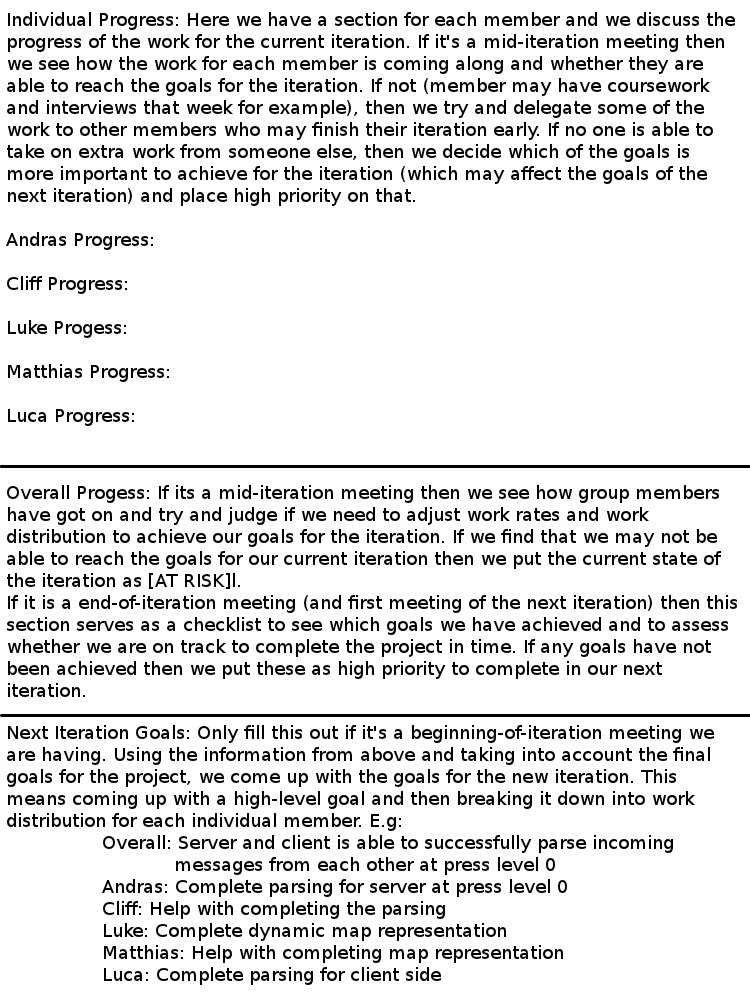
\includegraphics[width=100mm]{logbooktemplate.png}

\end{document}
